\section{Det Fysiske Lag}
\subsection{Teori}
I følgende teoriafsnit er der lagt vægt på Nyquist rasen, Goertzel, DTMF og C++ og SFML.

\subsubsection{Nyquist raten}
Hvis et signal skal analyseres, skal sampling frekvensen være større end to gange den frekvens signalet har, dvs:
\begin{equation}
f_s > 2 \times f_{max} \label{eq:nyq}
\end{equation}
Hvis dette krav ikke opretholdes, vil signal samplingen være påvirket af aliasing.

\subsubsection{Goertzel}
Goertzel er en speciel algoritme brugt til at udregne DFT (Diskret Fourier Transformation) koefficienter og signal spektrum, uden at bruge kompleks algebra som DFT.
\newline
Goertzel algoritmen er en filtreringsmetode for udregningen af DFT koefficienterne X(k) ved en bestemt frekvens bin, k.
\begin{equation}
k = \frac{f}{f_s} \times N \label{eq:goe}
\end{equation}

hvor f er den bestemte frekvens der ledes efter, og N er det totale antal samples der samples over.
\hfill \break

Goertzel filteret opererer med en indput sekvens x(n) i en kaskade af 2 stadier med en parameter f, som er den frekvens der skal analyseres.
\hfill \break

Filterets første stadie er et andensordens IIR filter:
\begin{equation}
s(n) = x(n) + 2 \times cos(2 \pi f)s(n-1)s(n-2) \label{eq:IIR}
\end{equation}

hvor der ved samplen $x(0)$ gælder at $s(-2) = s(-1) = 0$
\hfill \break

Filterets andet stadie er et FIR filter:
\begin{equation}
y(n) = s(n) - e^{2 \pi if} s(n-1) \label{eq:FIR}
\end{equation}

I en kaskade har filterets overføringsfunktion udseendet:
\begin{equation}
G(Z) = \frac{Y(Z)}{X(Z)} = \frac{1}{1-2 \times cos(\frac{2 \pi k}{N})z^{-1}+z^{-2}} \label{eq:of}
\end{equation}

Den kvadreret DFT koefficient X(k) ved en bestemt frekvens bin k, dvs. det enkeltsidet spektrum, er derfor givet således:
\begin{equation}
|X(k)|^2 = s(N - 1)^2 + s(N-2)^2 - 2 \times cos \bigg(\frac{2 \pi k}{N} \bigg) s(N-1) s(N-2) \label{eq:DTF}
\end{equation}

\subsubsection{DTMF}
DTMF står for: “Dual-tone multi-frequency signaling”, og er de kendte dial toner man kender fra telefonen. Hver tone er en kombinering af to sinusoidale signaler med frekvenser valgt ud fra et sæt af otte standardiserede frekvenser. Se figur \ref{fig:dtmf}
\begin{figure}[ht]
	\centering
	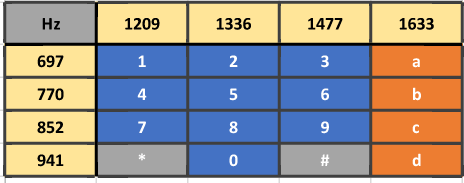
\includegraphics[width=10cm,height=10cm,keepaspectratio]{pictures/DTMF.png}
	\caption{DTMF toner}
	\label{fig:dtmf}
\end{figure}
\newline
Hos DTMF er det vigtigt at hver tone afspilles i længere end 40 millisekunde,r og at mellem hver tone er det en pause på 50 millisekunder.

\subsubsection{C++ og SFML}
C++ har pr. standard ikke funktioner til at afspille og optage lyd. Derfor blev biblioteket SFML installeret til at håndtere disse funktioner. SFML er en simple interface til de forskellige komponenter på ens pc, for at lette udviklingen af f.eks. spil og multimedia applikationer.
\newline
De klasser der bliver brugt fra SFML er:
\begin{itemize}
	\item \texttt{sf::Sound}
	\newline Bruges til at afspille lyd.
	
	\item \texttt{sf::\textcolor{dkgreen}{SoundBuffer}}
	\newline Lagring af audio samples der definere en lyd.
	
	\item \texttt{sf::\textcolor{dkgreen}{SoundRecorder}}
	\newline En abstrakt grund klasse til at optage lyd.
	
	\item \texttt{sf::\textcolor{dkgreen}{SoundBufferRecorder}}
	\newline En specialiseret \texttt{SoundRecorder}, der gemmer optaget lyd i en lyd buffer. 
\end{itemize}

\subsubsection{Optag}
Den første problemstilling projektet stødte på i forhold til optag, var at være i stand til at optage en DTMF tone og analysere optagelsen, hvorefter at fortælle hvilken tone der blev optaget.
\\
\newline
Før en optagelse kan finde sted, blev en samplingsfrekvens for optagelse nødvendigvis defineret og fastsat. Denne samplingfrekvens er yderst vigtig for projektet, eftersom denne samplingsfrekvens dikterer hvordan resten af det fysiske lag skal oprettes. 
\newline
Som et krav skal samplingsfrekvensen overholde Nyquist raten:
\begin{equation}
f_s > 2 \times f_{max}
\label{eq:samnyq}
\end{equation}

Den højeste frekvens hos en DTMF tone er 1633 Hz, derfor skal samplingsfrekvensen som minimum være 3267 Hz. Til projektet blev samplingsfrekvensen sat til 8000 Hz, eftersom det er en ofte brugt samplingsfrekvens ved implementering af DTMF genkendelse, og at den opretholder Nyquist raten.
\\
\newline
Projektets optagefunktioner hviler tungt på SFML bibliotekets klasser, \texttt{sf::\textcolor{dkgreen}{SoundRecorder}} og \texttt{sf::\textcolor{dkgreen}{SoundBufferRecorder}}, eftersom C++ egets bibliotek ikke tilbyder optagefunktioner.
\\
\newline
Projektets første løsning på at optage en DTMF tone og analysere optagelsen var en simpel løsning, der dog viste sig ikke at være tilstrækkelig for dette projekt.
\newline
En optagelse blev oprettet ved først at lave et objekt f.eks. \texttt{sf::\textcolor{dkgreen}{SoundRecorder}} optag.
\newline
Derefter startede SFML sin egen tråd og optog, når man brugte funktionen \texttt{optag.start(8000)} (8000 Hz for projektets samplingsfrekvens). Koden sættes til at sove den tid der skal optages, hvorefter at optagelsen stoppes med \texttt{optag.stop()}. Optagelsens information blev derefter hentet ved at lave en reference til optagelsens buffer \texttt{sf::\textcolor{dkgreen}{SoundBuffer} \&enBuffer}, derefter blev der oprettet en vektor af pointerer til bufferen \texttt{sf::\textcolor{dkgreen}{Int16*} samples = enBuffer.getSamples();}. Vektoren består nu af diskrete værdier for en optagelse, hvorpå der blev udført en DFT. Denne DFT vil således være i stand til at vise om en DTMF tone er til stede.
\newline
Første løsning på at optage en DTMF tone og analysere optagelsen er ikke forkert, den skabte umiddelbart noget kompleksitet, som projektet blev nødt til at tage højde for:
\begin{itemize}
	\item Løsningen kræver at optageren skal vide hvornår en afspiller af en sekvens af toner er færdig, eftersom analysen af optagelsen først kan finde sted efter en endt optagelse.
	
	\item DFT er en tung udregning. Den har et forhold der siger der er $N^2$ udregninger ved en DFT på N samples. Dvs. efter en optagelse på 10 sekunder sker der
	$$(10 sek \times 8000 Hz)^2 = 6.400.000.000$$
	udregninger, hvilket er en uheldig eksponentiel stigning for udregninger af længere optagelser.
\end{itemize}
Der blev derfor skrevet en klasse \texttt{MyRecorder.h} som arver funktionalitet fra \texttt{sf::\textcolor{dkgreen}{SoundRecorder}} klassen. Der arves 3 funktioner herfra:
\begin{itemize}
	\item \texttt{\textcolor{blue}{virtual bool} onStart()}
	
	\item \texttt{\textcolor{blue}{virtual bool} onProcessSamples(\textcolor{blue}{const} sf::\textcolor{dkgreen}{Int16*}samples, std::\textcolor{dkgreen}{size\_t} sampleCount);}
	
	\item \texttt{\textcolor{blue}{virtual void} onStop();}
\end{itemize}
\texttt{onStart()} og \texttt{onStop()} bliver kørt når et optagelses objekt af \texttt{MyRecorder.h} klassen f.eks. \texttt{\textcolor{blue}{MyRecorder} optag}, bliver startet med \texttt{optag.start()} eller sluttet med \texttt{optag.slut()}. Der kan så defineres start eller slut betingelser for en optagelse, såsom variable eller buffere der cleares.
\newline
\texttt{onProcessSamples()} er en funktion der bliver kørt automatisk og gentaget i samme tråd som optagelsen, afhængigt af hvad for et interval der sættes under \texttt{onStart();} (100 millisekunder pr. standard). Den bliver indlæst med parameteren \texttt{\textcolor{blue}{const} sf::\textcolor{dkgreen}{Int16*} samples}, dvs. en vektor med diskrete værdier for en optagelse, og hver gang funktionen kaldes er det de seneste nye værdier der ligger i vektoren. \texttt{onProcessSamples()} fortsættes med at blive kaldt hvis den returnerer true, og den stoppes hvis der returneres false.
\newline
Dvs. \texttt{MyRecorder.h} klassen kan optage og analysere data på én gang, hvilket løser problematikken om hvorvidt optageren skal vide hvornår den skal optage og afslutte en optagelse. Nu kan der f.eks. laves en starttone og en sluttone, som optageren kan opfange og derfra igangsætte bestemte kode dele.
\newline

Derudover blev klassen \texttt{Goertzel.h} skrevet som alternativ til en DFT udregning.
\newline
\texttt{Goertzel.h} klassen, som navnet antyder, benytter en Goertzel algoritme til at analysere vektoren med de diskrete værdier fra optagelsen. Jf. teori afsnittet, er Goertzel en smart måde hvorpå der kun udføres udregninger på de frekvens bins der ledes efter.
\newline
Dvs. at denne algoritme udfører langt færre udregninger i forhold til DFT og FFT(Fast Fourier Transform), netop fordi der ikke analyseres over alle samtlige DFT/FFT koefficienter. Dette gør at det ikke er noget problem at optage i længere.  
\hfill \break

Før Goertzel algoritmen kan implementeres er der nogle få ting der skal på plads først. Frekvens binsene skal regnes ud, jf. teori om frekvens bins, skal en samplingfrekvens vides og hvor mange samples der skal samples over. Samplingsfrekvensen er fastsat til 8000 Hz, dog skal det antal samples N som Goertzel analyserer over fastsættes. Der er dog nogle pointer ved fastsættelsen af N, jo større N bliver, desto større antal samples skal der udregnes over, men samtidig jo størrer N bliver, jo smallere bliver bredden af frekvens binen, dvs. at den bliver mere præcis. Det handler om at vælge en N, der ikke er for høj, da dette resulterer i tab af beregningshastighed, eller for lav, hvilket resulterer i tab af præcision.
\newline
Derudover må N ikke blive større end 400 samples, jf. teori om DTMF, da der er et tidsrum af 50 millisekunder mellem hver tone, grundet samplingsfrekvensen på 8000 Hz. Dette tidsrum er der for at forhindre, at en analyse af N samples fra en optagelse ikke foregår over et skift fra én tone til en anden.
\newline
Dette taget i betragtning blev N valgt til at være lig 300, eftersom det er tilpas højt for en tilfredsstillende bredde af frekvens binen (8000 Hz / 300 = 26,7 Hz, den må være helt op til 70 Hz før det skaber problemer), samtidig med det tidsrum som projektet faktisk har tilføjet mellem hver tone, kun er på 400 samples, dvs. 50 millisekunder.
\newline
Frekvens binen for hver DTMF frekvens er derfor udregnet, se tabel \ref{fig:tabel}, og kan bruges til implementeringen af \texttt{Goertzel.h} klassen.
\begin{figure}[ht]
	\centering
	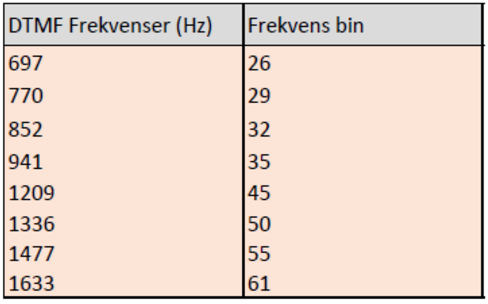
\includegraphics[width=10cm,height=10cm,keepaspectratio]{pictures/DTMFtabel.png}
	\caption{DTMF tabel}
	\label{fig:tabel}
\end{figure}

\subsection{Implementering}
Jf. teori om Goertzel vil filterets G(Z) realiserings struktur se således ud se figur \ref{fig:grs}. Denne realiserings struktur er blevet implementeret i \texttt{Goertzel} klassen ved hjælp af en for løkke, som kører en vektor af diskrete værdier, x(n), med N samples, igennem strukturens udregninger. Husk at ved $x(0) er s(-1) = s(-2) = 0$.
\begin{figure}[ht]
	\centering
	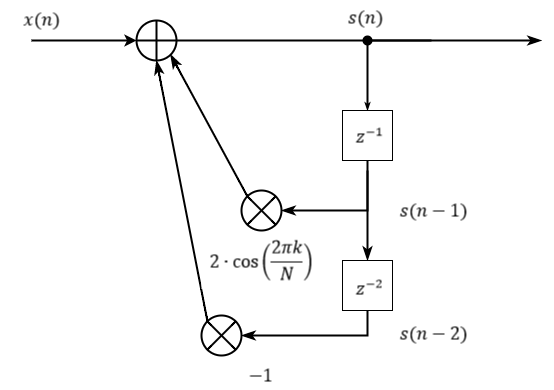
\includegraphics[width=10cm,height=10cm,keepaspectratio]{pictures/GRStruktur.png}
	\caption{Goertzel realiserings struktur}
	\label{fig:grs}
\end{figure} 
\newline
Denne for løkke er blevet implementeret således:
\begin{figure}[ht]
	\centering
	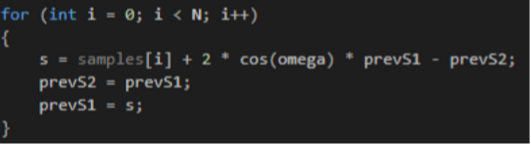
\includegraphics[width=10cm,height=10cm,keepaspectratio]{pictures/Forloop.png}
%	\caption{Goertzel realiserings struktur}
	\label{fig:forloop}
\end{figure} 
\newline
Derefter kan DFT koefficienten bestemmes for en givet frekvens bin k, fordi nu kendes værdierne for sekvensen $s(n)$ ved $s(N-1)$ og $s(N-2)$ (prevS1 og prevS2):
\begin{equation}
|X(k)|^2 = s(N-1)^2 + s(N-2)^2 - 2 \times cos\bigg(\frac{2 \pi k}{N}\bigg) s(N-1)s(N-2) \label{eq:DFTk}
\end{equation}

\texttt{Goertzel} klassens funktion er delt op i 2 metoder:
\begin{itemize}
	\item \texttt{\textcolor{blue}{int} detectFreqs(const sf::\textcolor{dkgreen}{Int16*} samples, \textcolor{blue}{int} K);}
	
	\item \texttt{\textcolor{blue}{int} findTone(const sf::\textcolor{dkgreen}{Int16*} samples);}
\end{itemize}
\texttt{detectFreqs()} bruger det ovenstående implementerede princip, hvorimod \texttt{findTone()} er en metode som bruger \texttt{detectFreqs()} til at gennemgå de tidligere nævnte frekvens bins og returnere en DTMF tone der er over en grænseværdi i forhold til DFT koefficienten. Tonerne er blevet defineret som integers fra 0 til 15, og en grænseværdi er nødvendig fordi en tilfældig støj der rammer en frekvens bin kan blive opfanget.
\newline
\texttt{MyRecorder} har seks metoder:
\begin{itemize}
	\item \texttt{\textcolor{dkgreen}{vector} <\textcolor{blue}{int}> getBesked();}
	
	\item \texttt{\textcolor{blue}{bool} getNyBesked();}
	
	\item \texttt{\textcolor{blue}{bool} getBeskedBegyndt();}
\end{itemize}
\texttt{getBesked()} er den metode der kaldes for at hente de DTMF toner, som blev optaget.
\newline
\texttt{getNyBesked()} og \texttt{getBeskedBegyndt()} er metoder til at kalde boolske udtryk, som bliver brugt til at manipulere og styre \texttt{MyRecorder}.
\begin{itemize}
	\item \texttt{\textcolor{blue}{virtual bool} onStart();}
	
	\item \texttt{\textcolor{blue}{virtual bool} onProcessSamples(\textcolor{blue}{const} sf::\textcolor{dkgreen}{Int16*} samples, std::\textcolor{dkgreen}{size\_t} sampleCount);}
	
	\item \texttt{\textcolor{blue}{virtual bool} onStop();}
\end{itemize}
\texttt{onStart()}, \texttt{onProcessSamples()} og \texttt{onStop()} fungere som tidligere nævnt, dog kaldes \texttt{findTones()} fra \texttt{Goertzel} klassen under hver \texttt{onProcessSamples()} kald, netop fordi der skal optages og analyseres samtidigt.
\hfill \break

For at gøre det nemmere at skrive funktionaliteterne for klasserne \texttt{MyRecorder} og \texttt{Goertzel}, blev der taget udgangspunkt i sekvensdiagrammet SE BILLEDE BILAG WHATEVER. 
\newline
\texttt{MyRecorder} bliver kaldt af \texttt{ToneKonvertering} i det, at det er den klasse som skal modtage beskeden, som består af en vektor af toner, som derefter bliver pullet op igennem applikationens forskellige lag.
\newline
Når \texttt{ToneKonvertering} kalder \texttt{MyRecorder}, blev funktionaliteten for, hvorledes om en optagelse fanger en besked eller ej og om hvor lang en optagelse er, nødt til at blive implementeres under \texttt{ToneKonvertering}s metoden \texttt{returnBitString()}.
\newline
Der er blevet implementeret en while løkke, som kører enten indtil der er gået 10 sekunder, eller at en sluttone på en besked blev opfanget vist i  figur \ref{fig:returnbitstrengwhile}.
\begin{figure}[ht]
	\centering
	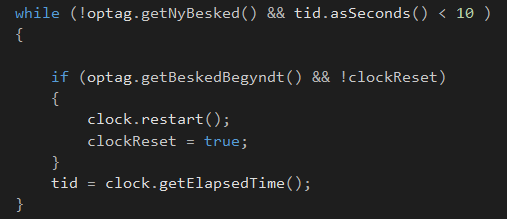
\includegraphics[width=10cm,height=10cm,keepaspectratio]{pictures/Returnbitstrengwhileloekke.PNG}
	\caption{While løkke}
	\label{fig:returnbitstrengwhile}
\end{figure}
 Der er en if sætning der tester for, om en starttone er blevet hørt, hvis den fanges, skal timeren tælle til 10 forfra. Herefter returneres en vektor med alle de optagede toner. Dvs. at optagelsen altid vil være maks. 10 sekunder lang, hvilket resten af applikationen tager højde for.
\newline
\texttt{MyRecorder} starter en optagelse med samplingsfrekvensen 8000 Hz i dens egen tråd, når metoden \texttt{start(8000)} bliver kaldt. \texttt{onProcessSampling()} kaldes hvert 10’ende millisekund i denne tråd. Under hvert kald bliver de optagede samples analyseret af Goertzel, som returnere tonen for de samples. Denne tone gemmes i \texttt{resusltatVektor}’en, som indeholder de toner, som hele optagelsen opfangede. Udover dette, sker der en mindre sortering af tonerne der optages under \texttt{onProcessSampling()} (dette fremgår ikke af sekvensdiagrammet). Tonerne skal ikke gemmes i \texttt{resusltatVektor}’en medmindre der først har været en starttone. Ved en sluttone stoppes \texttt{onProcessSampling()} for at blive kaldt igen, medmindre en helt ny optagelses session startes. Start og stop tonerne er blevet  defineret som tone 15 (D) = start og tone 14 (\#) = stop. Disse to toner bliver tilført som flag og taget højde for i de øvrige lag.

\subsection{Diskussion}
I projekts tidlige stadie var der en del usikkerhed omkring pålideligheden af \texttt{MyRecorder} og \texttt{Goertzel} klassens optagede besked, eftersom det virkede til at der var en tilfældig bouncing effekt mellem et skift af tone under optagelsen. Selv midt i en tone optagelse var der chance for et bounce. Ved en forholdsvis lav sendehastighed, 4 toner pr. sekund, var bouncing effekten tilstede, dog reduceret.
\newline
Dette var ikke et stort problem ved starten af projektet, eftersom der oprindeligt blev sendt med en hastig af 8 toner pr. sekund. De højttalere som blev udleveret med projektbeskrivelsen inducerer mere af denne formodede bouncing, i forhold til nogle af projektets medlemmers private højtalere, som der blev testet på til at starte med.
\newline
Højttalernes kvalitet har derfor vist sig at have påvirkning på hvor et rent DTMF signal der laves.
\hfill \break

Udviklingen af et filter til optagelse havde været en mulig løsning på højttalernes kvalitet, men i projektet blev der implementeret en debouncer i \texttt{MyRecorder} klassen, for at sikre der ikke sker fejl under behandlingen af optagelsen. Debounceren er en forholdsvis stor debouncer. Den tjekker for de to forrige værdier, og tjekker om signalet er færdig med at bounce. Dvs, at projektet kræver at en tone skal opfanges tre gange før den godtages. Denne debouncer gør, at kommunikation med DTMF i projektet bliver betydeligt langsommere, fordi en tone skal være til stede 3 gange så lang tid før tonen bliver accepteret. For projektet er sendehastigheden blevet langsommere, 4 toner pr. sekund.
\hfill \break

Det har vist sig ved slutningen af projektet, at den bouncing effekt der opleves, højst sandsynligt skyldes en fejl i \texttt{Goertzel} klassens metode \texttt{findTone()}. En grænseværdi er ikke blevet initialiseret korrekt (der er ingen grænseværdi for en af sorterings løkkerne i metoden), men grundet tidspres er det en fejl der rettes i en senere udgivelse af applikationen, fordi en udvidet testfase skal udføres, og hele applikationen skal opdateres til at arbejde med de opnåede resultater fra testfasen.

\subsection{Afspil}
Projektet har den problemstilling, at der skal afspilles en forudbestemt sekvens af toner, i forhold til en besked.
\newline
Al funktionalitet som vedrører afspilning af DTMF toner er afhængig af SFML bibliotekets klasser \texttt{sf::\textcolor{dkgreen}{Sound}} og \texttt{sf::\textcolor{dkgreen}{SoundBuffer}}, eftersom C++ egets bibliotek ikke tilbyder afspilning af DTMF toner.
\hfill \break

Før afspilning kan finde sted, skal der fastsættes en samplingsfrekvens, samt hvor mange samples pr. DTMF tone der er i en afspilning. Der kunne med fordel tages udgangspunkt i optage afsnittet for projektet, og benytte den samme samplingsfrekvens - 8000 Hz . Derudover skal afspil nødvendigvis afspille i den hastighed som applikationen kan optage med, dvs. 4 toner pr. sekund - så 2000 samples pr. tone.
\newline
De ønskede DTMF toner der skal afspilles (hvis det er rå data), skal indlæses i en vektor af diskrete værdier. Vektoren er defineret som :
$$\texttt{\textcolor{dkgreen}{vector}<sf::\textcolor{dkgreen}{Int16}>raw1;}$$
\newline
\texttt{raw1} er her vektoren med datatypen \texttt{signed \textcolor{dkgreen}{Int16}}. Dvs. at amplituden for en diskret værdi kan maks være af størrelsen $\frac{2^16}{2}$. Data’en for en DTMF tone kan med fordel laves ved hjælp af en for løkke, som lægger to sinusoidale funktioner sammen, bestående af de frekvenser som indgår i DTMF tonen. Se figur \ref{fig:dtmfkode} for kode eksempel.
\begin{figure}[ht]
	\centering
	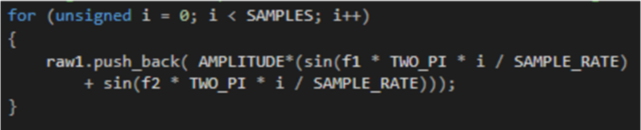
\includegraphics[width=15cm,height=25cm,keepaspectratio]{pictures/DTMFkode.png}
	\caption{Kode eksempel}
	\label{fig:dtmfkode}
\end{figure}
\newline
Denne vektor skal indlæses i et buffer objekt lavet af \texttt{sf::\textcolor{dkgreen}{SoundBuffer}} klassen. Bufferen skal også indlæses med en integer, for hvor mange samples der er i vektoren, og hvilken samplingsfrekvens afspilningen skal have. Derefter kan et \texttt{sf::\textcolor{dkgreen}{Sound}} objekt laves f.eks. \texttt{sf::\textcolor{dkgreen}{Sound}} lyd, dette objekt skal indlæses med bufferen, som indeholder den information som \texttt{sf::\textcolor{dkgreen}{Sound}} objektet skal afspille. Dette gøres med metoden \texttt{lyd.setBuffer(buffer)}. \texttt{sf::\textcolor{dkgreen}{Sound}} objektet kan nu afspilles med metoden \texttt{lyd.play()}, hvorefter applikationen sættes til at sove den tid afspilningen tager.
\hfill \break

Projektets første løsning på at afspille en DTMF tone, var en simpel men utilstrækkelig løsning. Den brugte ovenstående metode til at afspille toner med, ved oprettelse af et objekt f.eks. tone(frekvens1, frekvens2), som blev kørt igennem ovenstående for løkke. \texttt{raw1} blev derefter afspillet. En sekvens af toner, var derfor en sekvens af tone objekter der først skulle oprettes, og derefter sendes til afspilning en af gangen. Hvis en tone indgik flere gange i en sekvens, så blev den oprettet igen hver gang. Første løsning skabte derfor følgende problemstillinger:
\begin{itemize}
	\item Dette foregik i samme klasse, og skabte low cohesion eftersom det at afspille og generere toner er 2 forskellige ting.
	
	\item Det en langsom process, som var tydelig under projektets test stadie, og havde indflydelse på kvaliteten af en sekvens af afspilninger.
	
	\item Jf. teori om DTMF, mangler der en pause på 50 millisekunder mellem hver tone.
	
	\item Metoden skal have tone objekter som input, hvilket de øvre lag ikke kan tilbyde.
\end{itemize}
Der blev derfor skrevet to klasser til at løse problemstillingerne, \texttt{Afspil.h} og \texttt{Tone.h}. \texttt{Afspil} klassens ansvar er udelukkende at afspille data, og \texttt{Tone} klassen står for at oprette denne data.

\subsubsection{Implementation}
For at gøre det nemmere at implementere ovenstående funktionalitet blev der taget udgangspunkt i FIGUR SEKVENSDIAGRAM LORT. 
\newline
Tone klassen opretter objekter som består af 2 frekvenser
\begin{itemize}
	\item \texttt{Tone(\textcolor{blue}{int} frekvens1, \textcolor{blue}{int} frekvens2);}
\end{itemize}
Hvert objekt køres igennem den før nævnte sinusoidale for løkke, og opretter data for hvert tone objekt. Disse data kan så tilgås ved følgende metode som er blevet skrevet i \texttt{Tone} klassen:
\begin{itemize}
	\item \texttt{\textcolor{dkgreen}{vector}<sf::\textcolor{dkgreen}{Int16}>getRaw();}
\end{itemize}
\hfill \break
\texttt{Afspil} klassen har tre metoder:
\begin{itemize}
	\item \texttt{sendData({\textcolor{dkgreen}{vector}}<\textcolor{blue}{int}>input)}
	
	\item \texttt{makeRaw0(\textcolor{dkgreen}{vector}<\textcolor{blue}{int}>input)}
	
	\item \texttt{afspilToner(\textcolor{blue}{int} længdeAfElementer)}
\end{itemize}
\texttt{sendData()} er en offentlig metode, som sørger for at sende en besked, ved at bruge \texttt{makeRaw0()} og \texttt{afspilToner()}. Inputtet fra de øvrige lag, er en sekvens af integers, som symboliserer toner. 
\hfill \break

\texttt{makeRaw0()} sørger for, at lave en ny vektor, \texttt{\textcolor{dkgreen}{raw0}}, med sekvenser af tone data. \texttt{makeRaw0()} slår op i vektoren \texttt{\textcolor{dkgreen}{dtmfToner}} i \texttt{Afspil} klassen når den får en besked den skal afspille, og kopier indholdet over i \texttt{\textcolor{dkgreen}{raw0}} det kan ses i \ref{fig:makeRaw0}.
\begin{figure}[ht]
	\centering
	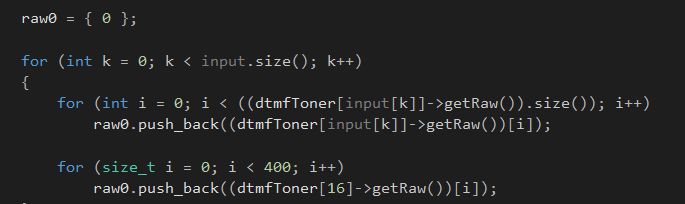
\includegraphics[width=15cm,height=25cm,keepaspectratio]{pictures/makeRaw0.PNG}
	\caption{Metode makeRaw0}
	\label{fig:makeRaw0}
\end{figure}
 \texttt{\textcolor{dkgreen}{dtmfToner}} består af tone objekter og er sorteret fra 0 til 15, som er de integers der symboliserer hver tone. Hver gang \texttt{makeRaw0} har kopieret en tones data til vektoren, så lægger den 400 samples af tone 16 oven i, (400 samples er 50 millisekunder), netop fordi der skal være en pause af 50 millisekunder mellem hver tone jf. teori om DTMF.
\newline
\texttt{afspilToner()} afspiller altid \texttt{\textcolor{dkgreen}{raw0}}, dog skal metoden vide hvor mange elementer der afspilles som input.
\hfill \break

De tidligere nævnte problemstillinger er derfor løst. Der er to klasser med hver deres ansvar. Tone objekter bliver kun oprettet en gang, nemlig ved applikationens start, så det går betydeligt hurtigere at generere en afspilning. Der er blevet tilføjet de 50 millisekunders pause. De øvrige lag skal kun give en vektor af integers for at igangsætte en afspilning.

\subsubsection{Disussion}
Afspilning af DTMF toner var en af projektets første problemer der blev undersøgt. Der var ikke tænkt over hvordan applikationen optog endnu, og det var først efter at optage delen af applikationen kom på plads, at afspilnings delen blev revurderet. Derfor var en afspilning i starten af projektet indlæst med en samplingsfrekvens på 44100 Hz (cd kvalitet) uden videre tanke for, at det ville skabe lange udregningstider. Et alternativ, projektet kunne have brugt, var at have lydfiler for hver tone inkluderet i applikationen, disse lydfiler kunne afspilles med SFML i forhold til en besked.